\chapter{Improved Ensemble}
In the past chapter, we showed that a few changes can lead to some significant improvements in multi-step forecasting accuracy when ensemble Bayesian Combined Forecasting is applied to our traffic datasets.  This chapter describes more in depth some of the problems with BCF.  We look at some related work into potentially solving these problems through the identification and modeling of activities and finally introduce a new ensemble forecasting technique which solves these problems.  

\begin{figure}[!b]
	\begin{center}
		\subfigure[] {
			\includegraphics[width=0.49\textwidth]{sample_residual_event_804.png}
		}
		\subfigure[] {
			\includegraphics[width=0.49\textwidth]{sample_residual_event_6024.png}
		}
	\end{center}
	\caption{Two similar events occurring at different time in the same residual dataset.}
	\label{fig:sample_residual_events}
\end{figure}


%%%%%%%%%%%%%%%%%%%%%%%%%%%%%%%%%%%%%%%%%%%%%%%%%
%Need for another ensemble forecaster
%%%%%%%%%%%%%%%%%%%%%%%%%%%%%%%%%%%%%%%%%%%%%%%%%
\subsection{The need for another ensemble forecaster}
When analyzing the residual datasets of these ensemble forecasts, we noticed a fundamental problem with our forecaster.  In the residual forecasts of BCF and many of the forecasting algorithms, the resulting residual forecast would still have many repeated misforecasts that could not be explained by random noise.  As alluded to in Chapter 1, these repetitive misforecasts may come from large human controlled scheduled events (such as sporting events, public celebrations, or in the case of buildings meetings) or they may be from uncontrolled and unscheduled events (such as weather or traffic accidents).  

\begin{figure}[!t]
	\begin{center}
		\subfigure[] {
			\includegraphics[width=0.49\textwidth]{denver_bcf_residual_15.png}
		}
		\subfigure[] {
			\includegraphics[width=0.49\textwidth]{denver_bcf_residual_26.png}
		} \\
		\subfigure[] {
			\includegraphics[width=0.49\textwidth]{denver_bcf_residual_32.png}
		}
		\subfigure[] {
			\includegraphics[width=0.49\textwidth]{denver_bcf_residual_38.png}
		}
	\end{center}
	\caption{Scaled histogram of IBCF residual values for the Denver traffic dataset at various time steps.  The red line is the corresponding best fit Normal distribution.  Notice how in all plots there exist data points which exist after the tails of the Normal distributions have approached zero.}
	\label{fig:denver_bcf_residual}
\end{figure}

~\ref{fig:sample_residual_events} shows two of these events occurring.  Such an event clearly occurs outside the normal behavior noise of our data.  The light red region in this image represents the one standard deviation boundary for the residual data.  From chapter 4, we know that BCF residual data tends to be normally distributed per daily time step.  The residual datasets from each time step pass the one-sample Kolmogorov-Smirnov \cite{Marsaglia2003, Lopes2007} test for normality ($p \ge 0.1$).  Assuming this data is truly normally distributed then the odds of getting even one such datapoint outside the $\pm 3 \sigma$ should occur roughly 1 in every million data points.  Yet, in our Denver traffic data, we had 22 such instances in the testing dataset alone ($N \approx 12000$).  

~\ref{fig:denver_bcf_residual} shows these results graphically.  In this figure, a histogram of the data from four different time steps from the Denver traffic dataset, overlaid with the corresponding best fit normal distribution.  In each image the same pattern appears.  Residual values around the mean and on the tails tend to occur with a greater frequency than would be suggested by a normal distribution.  Values around the mean are not the problem.  These values correspond to accurate forecasts.  Values around the tail however are problematic and are further evidence of large events being one of the causes of noise in our residual data.

The unlikely existence of these events along evidence that the remaining residual time series behaves as a white noise Gaussian process provides evidence that these events are likely not due to natural noise and instead due to other factors.  The remainder of this chapter discusses ways to identify and model these anomalous events along with providing an algorithm for using these events to improve our forecasting algorithm.


%%%%%%%%%%%%%%%%%%%%%%%%%%%%%%%%%%%%%%%%%%%%%%%%%
%Overview ABCF
%%%%%%%%%%%%%%%%%%%%%%%%%%%%%%%%%%%%%%%%%%%%%%%%%
\subsection{Bayesian Combined Forecasting with Activity and Anomaly Modeling (ABCF)}

\begin{wrapfigure}{L}{0.3\textwidth}
\centering
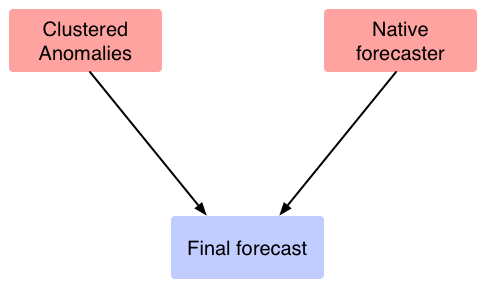
\includegraphics[width=0.25\textwidth]{simple_approach_overview.png}
\caption{Extremly high level overview of our approach}
\label{fig:highlevel_overview}
\end{wrapfigure}

As outlined in the introduction, we return here to a brief discussion of our approach.  The structure of non-Gaussian anomalies in the residual datasets of our forecasts leads us to explore if models of these anomalies can be used to improve our forecasts.  We propose a hybrid ensemble approach which can be applied to any forecaster and may lead to improved results.  

A high level view of our approach is detailed in \ref{fig:highlevel_overview}.  Given any forecaster trained forecaster, we extract a set of residual data.  Searching this residual dataset, we next attempt to extract and model the most representative set of anomalous events.  From \ref{fig:sample_residual_events}, we know that for our traffic systems - and we believe for many other human controlled traffic systems - that these events are not unique and are likely to repeat with similar behavior.  These anomalous events are then used as the basis of an ensemble forecaster combined with a zero mean background model which represents the native forecaster.  

In section \ref{sec:abcf} we introduce a recursive ensemble forecaster which uses clustered anomalies as inputs and works on the residual dataset of any given native forecaster.  Finally, using both the anomaly ensemble inputs and the native forecast, we combine the results to produce a final forecast.  


%%%%%%%%%%%%%%%%%%%%%%%%%%%%%%%%%%%%%%%%%%%%%%%%%
%Background literature
%%%%%%%%%%%%%%%%%%%%%%%%%%%%%%%%%%%%%%%%%%%%%%%%%
\subsection{Background Literature on Activity Recognition and Anomaly Detection}
To construct our approach we need to identify and model these anomalous events.  Considerable work has been done in the field of time series anomaly detection, however this work is typically limited to anomaly detection and classification.  Anomaly modeling as used for improved forecasting seems to have limited results in the forecasting literature.  We believe that this limited amount of anomaly modeling is often due to the nature of anomalies, either they are random and seemingly often times difficult to predict as is the case with stock market anomalies ~\cite{Kontonikas2013, Thushara2014} or they require some immediate attention and thus forecasting is an inappropriate response to the anomaly.  Such a situation arises frequently in network data monitoring.  Detection and classification of network anomalies help to determine potential network attacks \cite{Tartakovsky2013, Gogoi2011} and allow for preventive measures to take place, but forecasting network traffic during these anomalies is of little utility.  
   
Our anomalies tend to be repetitive and multiple time steps in length.  Data of this form is very closely related to another field of time series data analysis - that of activity recognition.   Due broad nature of this term and the breadth of research on anomaly detection, we briefly discuss some of the ways in which time series anomaly detection and activity recognition has been utilized in the past as a way to familiarize the reader with a discussion of the literature.  This review is not meant to be a complete list of all works in these fields, but instead gives an overview of the types of work done in this field so that we may better contrast previous work with our approach.

\bigskip
\noindent \textbf{Anomaly Detection} \\
From Eamon Keogh, a prominent researcher in time-series anomaly detection, a reading or series of readings is anomalous in a time-series if the 

\begin{quote}
"frequency of occurrences differed substantially from that expected, given previously seen data."
\end{quote}

A common method of anomaly detection is through the use of tools to assist in visual identification \cite{Stoffel2013, Lakhina2004, Shi2012}.  Tools have been extensively developed for network anomaly detection.  Such tools allow network administrators and researchers to quickly identify and potentially classify anomalies in the form of certain network attacks.  This is done by giving providing graphs, and overlay visualizations which make the identification of patterns more apparent.  Through the use of these tools, network administrators are able to quickly respond to  various attacks and minimize the potential damage to the network.  Visual assistance tools for anomaly detection do not provide modeling and forecasting of anomalies and thus are of little utility for utilizing anomalies to improve traffic system forecasting.   

Another common technique for anomaly detection within time series data is known as change point (or step detection).  Originally developed for statistical quality control, the cumulative sum control chart (CUSUM) \cite{page1955} is a classic algorithm for detecting changes in the mean of a time series.  It involves the calculation of a cumulative sum of the weighted observations.  When this sum exceeds a certain threshold value, a change is value is declared.  A problem with this approach is that the thresholds need to be known a priori.

The field of change point detection is quite heavily researched.  Researchers have developed algorithms for most types of data and computational scenarios.  There are algorithms to detect changes in time series mean, changes in variance and changes in distribution from the exponential family \cite{Dessein2013}.  These algorithms can operate offline, online \cite{Tartakovsky2013}, top down, bottom up and globally.  An excellent summary of current state of the art in change point detection spanning all major formulations (Bayesian, minimax, and generalized Bayesian) is found in \cite{Polunchenko2012}

TODO CLEAN UP CHANGE POINT TECHNIQUES

Spectral Methods:
Widely used in other fields to distinguish hidden patterns and trends from a noisy background.
\cite{Barford2002}

\bigskip
\noindent \textbf{Individual Activity Modeling and Recognition} \\
Work in activity recognition has focused on recognizing either individual activities or group activities.  In this section we describe many of the individual activity recognition techniques.  One common type of individual activity recognition is from wearable sensors such as accelerometers or RFID tag readers.  This type of work is almost always supervised and the goal is to map sensor readings to a comprehensible activity such as dish washing or tooth brushing \cite{Wang2009,Bao2004}.  While some of this has potential applications to our goals, much of it is not applicable as the focus is typically on recognizing activities from fully labeled datasets.  Authors from this field have used many of the standard machine learning models: decision trees \cite{Bao2004}, support vector machines \cite{Krishnan2008,Bao2004,Lustrek2009}, naive Bayes \cite{Bao2004,Lustrek2009}, nearest neighbor \cite{Bao2004,Lustrek2009}, and hidden Markov Models (HMM) \cite{Wang2009,Oliver2002}.  Comparisons amongst models have shown that performance is data dependent and that no one model appears to be best for all types of activities \cite{Bao2004,Lustrek2009}

Huynh \cite{Huynh2008} used a naive Bayes classifier in a different way for wearable sensor individual activity recognition.  Instead of using it to describe activity, it was used as a dimensionality reduction technique the results of which were the basis for a dictionary in latent Dirichlet allocation \cite{Blei2003}.  The topics generated from latent Dirichlet allocation are then clustered using k-means.  Each of these clusters represents a single activity.  This clustering approach proved effective for the recognition of repeated activities throughout the day, but due to its reliance of a fixed ratio of latent Dirichlet allocation projected topics, it is likely that recognizing combinations of activities will prove problematic.

To account for activities of varying time lengths, probabilistic suffix trees \cite{Hamid2007} have shown to be an effective model for activities.  Trees are trained using all sequential subsets of an input sequence and a total model is then created from the set of trees using AdaBoost \cite{Freund1996}.  The performance level of suffix trees seems to be highly noise dependent.  \cite{Hamid2006} compared HMMs with suffix trees and found that suffix trees out performed HMMs when the data was without noise, but as the noise increased HMMs performed increasingly better, eventually surpassing the performance of suffix trees.

\bigskip
\noindent \textbf{Group Activity Modeling and Recognition} \\
There are a limited number of publications that exist on group activity modeling recognition using a large number of sensors.  Within this problem domain the challenges to solve are different due to the type of data collected and due to group activities typically occurring over multiple sensors.  The data from the sensors is normally binary which leads to ambiguity determining true counts and direction of motion for cars or people.  Despite this ambiguity it is relatively easy to automatically construct the topology of the sensors \cite{Wren2003, Wren2006a}.  Empirically it seems as though this topology roughly correlates to the spatial distribution of the sensors.  We will use this spatial information later to better model events which occur over multiple sensors.
	
HMMs have been used as a model for learned activities.  These models are used to build a tree \cite{Minnen2004, Wren2006a} with each level described by a model with a different number of hidden nodes meaning that model accuracy is roughly correlated to tree depth.  At the top of the tree are simple models used to describe gross activities.  The leaves of the tree are highly complex models describing specific activities.  This tree structure has the advantage of being computationally efficient while maintaining accuracy on par with other techniques based on clustering of HMMs \cite{Clarkson1999}.  
	
In a method similar to the HMM tree, work has been done to create a hierarchy of fixed filters based on possible sensor topologies \cite{Wren2006}.  At each level of the hierarchy, the number of sensors and the amount of time history increases.  The probability of occurrence of each fixed arrangement is then computed when all levels are created, the resulting model represents the total classifier.  The usage of fixed sensor topologies is highly environment dependent and the fixed time lengths with each level of the hierarchy are likely too restraining for the types of activities we expect to observe.  

From the results of all activity recognition papers, it appears that approaches which show the most promise tend to use a model which allows comparison of inputs with various time lengths.  Also, hierarchical techniques tend to perform better than multiple models of equal complexity.  In defense of these general observations is the work of Huynh \cite{Huynh2005} who found that empirically for his problem, there is not a single feature or time window of past history that will perform best for all activities.  Instead each activity is best modeled by a set of features and length of time unique to that activity.  Huynh postulates that his finding is true of most activity recognition problems and concludes that his finding demonstrates a fundamental flaw present in many of the activity recognition techniques to be described as the typical approach is to search for an optimal set of activity models for a fixed feature space and window of time.


\subsection{Anomaly extraction and representation}
As we showed earlier in this section with ~\ref{fig:denver_bcf_residual}, the tails of the best fit Gaussian for the BCF residual random variable tend to have larger than expected likelihoods.  These unlikely residuals do not appear to be completely random.  From a review of the literature, we know that there are numerous methods to extract and model this data.  For our work, we propose a simple extraction technique and then model the data according to a time-series mixture of Gaussians.  This method allows us to impart a probabilistic behavior to our anomaly models.  Such behavior is essential to our eventual forecasting technique.

\begin{figure}[]
	\begin{center}
		\subfigure[] {
			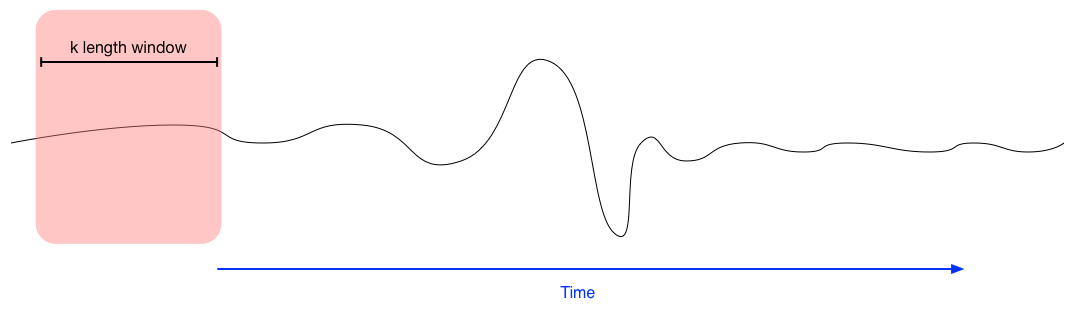
\includegraphics[width=0.50\textwidth]{slide_window_1.png}
		}
		\subfigure[] {
			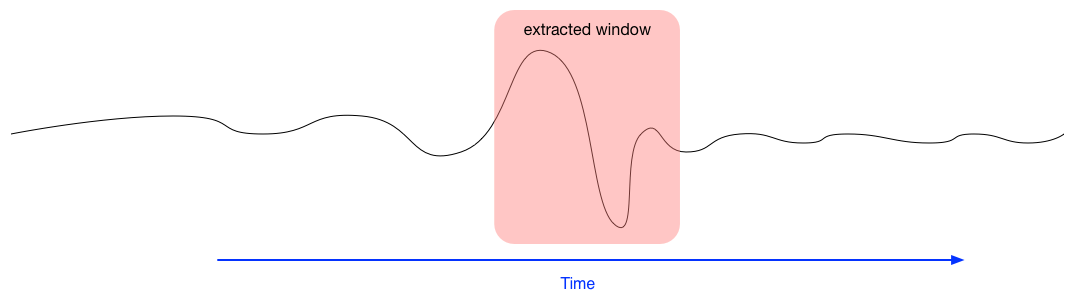
\includegraphics[width=0.50\textwidth]{slide_window_2.png}
		}
	\end{center}
	\caption{Demonstration of a fixed width sliding window looking for locally maximal deviations from background behavior.}
	\label{fig:sliding_window}
\end{figure}

\bigskip
\noindent \textbf{Sliding window data extraction} \\
Given time series of residual data, we extract the top $k\%$ of the maximum residual data as measured by a fixed length sliding window.  ~\ref{fig:sliding_window} demonstrates visually our method of potential candidate data segments to model.  In this example, the fixed length window is slid along a time series and windows with large total residual deviation are selected. 

TODO FINISH THIS ALGORITHM
\begin{algorithm}
  \caption{Algorithm for candidate data extraction}
    \label{alg:dataextract}

  \begin{algorithmic}
    \Statex \Comment { \%comment: servers[] contains the index of servers whose         data rate are sorted in descending order\%}
    \State servers[]= index(of all servers) 
    \State serverIndex[]=servers[0..K]
    \State linearlyIndependentServerIndex[]=0
    \State $[Z] \leftarrow 0$
    \For  {$i=0$ to $serverIndex.length$} 
    \Statex\Comment{ \%comment: find the equation corresponding the serverIndex        from the mapping at the File Server\%} 
    \State        $eqn= equation(serverIndex[i])$ 
    \Statex\Comment{ \%comment: try insert equation into Z using OFG\%} 

    \EndFor end for 
    \While{ ( linearlyIndependentServerIndex.length!=K ) } 
    \Statex\Comment{\%comment: remove all the server index which were not inserted in Z\%}  
    \State temp[]=serverIndex[]-linearlyIndependentServerIndex 
    \If{  (linearlyIndependentServerIndex.length=K) }
    \State break
    \EndIf  
    \EndWhile  
  \end{algorithmic}
\end{algorithm}

Algorithm \ref{alg:dataextract} describes precisely our approach.  The input parameter $k\%$ is chosen empirically for each dataset and underlying forecasting model.  The effects of this parameter $k$ are discussed later.  A sample of the top 10\% extracted residuals for the Merl dataset is displayed in \ref{fig:extracted_residuals}

Future work should allow for anomaly models which are non-constant in length.  An interesting possibility for the extraction and molding sparse dictionary learning. For this work however, we believe that constant length anomaly extraction is sufficient to show the strength of our combined forecasting approach.


\begin{figure}
	\begin{center}
		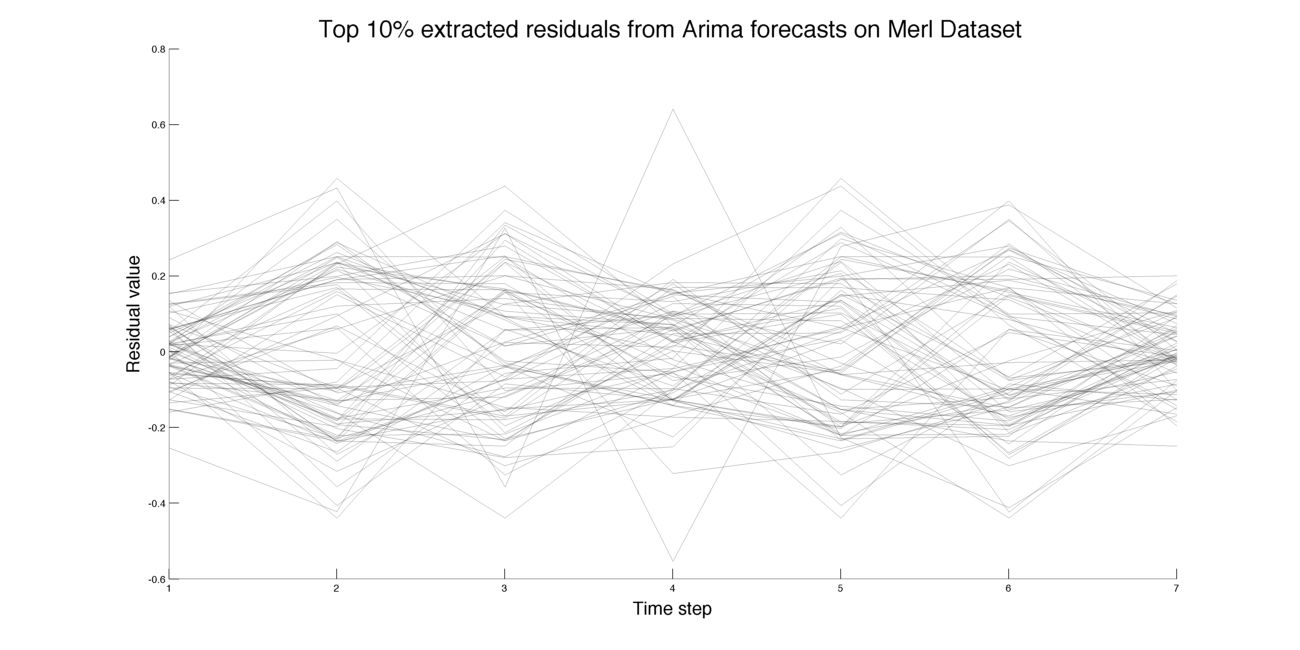
\includegraphics[width=0.90\textwidth]{arima_abcf_extracted_residuals_Merl.png}
	\end{center}
	\caption{Extracted residuals from the Merl dataset using the sliding window extraction method with window length of 7}
	\label{fig:extracted_residuals}
\end{figure}



\subsection{TSMG derivation}
TODO Move this derivation to the APPENDIX AND JUST DISCUSS OUR MODEL APPROACH HERE.

Discuss the silhouette score for best fit clusters.


A mixture of Gaussians is a strongly supported stochastic data clustering technique used in activity recognition.  Traditionally, a mixture of Gaussians is implemented for either a one dimensional time series (CITE PAPER TO SUPPORT THIS) or for data vectors with no time element.  Here we combine the two approaches, creating a mixture of Gaussians for multi-dimensional time series data.  While this approach has not yet been implemented, based on the success of mixture of Gaussians in other domains, we expect good results.

The goal of mixture of Gaussians is to find a set of models which will maximize the log likelihood of the parameters of some models to the dataset.  Given dataset $\{x^{(i)}\}$ we maximize
\begin{equation}
\ell(\theta) = \sum_{i = 1}^{\bf M}log\{p(x^{(i)}|\theta)\}
\end{equation}
\noindent 
where ${\bf M}$ is the total number of time series instances.

The expectation maximization (EM) algorithm is commonly used to maximize dataset likelihood.  To use this algorithm we need to define a set of variables
\begin{equation}
w_{k}^{(i)} = p(z = k|x^{(i)})
\end{equation}
\noindent
where ${\bf K}$ is the total number of Gaussians to train and $k$ is an index of ${\bf K}$.  

The general equation for the likelihood of the models is: 
\begin{equation}
\label{eq:em_likelihood}
\ell(\theta|x) = \sum_{i = 1}^{{\bf M}}\sum_{k = 1}^{{\bf K}}w_{k}^{(i)}\log \{ \frac{p(x^{(i)}|z=k)p(z = k)}{w_{k}^{(i)}} \}
\end{equation}

In the traditional mixture of Gaussians algorithm each model is ostensibly a Gaussian.  To make this algorithm work with multi-dimensional time series, we define the models instead by
\begin{equation}
\label{eq:model}
p(x^{(i)}|z = k) = \prod_{n = 1}^{{\bf N}}\mathcal{N}_{n}(x^{(i)})
\end{equation}
\noindent
where ${\bf N}$ is the length of each time series instance.  Thus our model for each time series is ${\bf N}$ independent multivariate Gaussians.

Combining equations~\ref{eq:em_likelihood} and~\ref{eq:model} gives the following log likelihood
\begin{equation}
\label{eq:em_combined}
\ell(\theta|x) = \sum_{i = 1}^{{\bf M}}\sum_{k = 1}^{{\bf K}}w_{k}^{(i)}\{ \log\frac{p(z = k)}{w_{k}} + \sum_{n = 1}^{{\bf N}} \log \mathcal{N}_{n}(x^{(i)})\}
\end{equation}

\textbf{E-Step}
The E-step hardly changes from the traditional EM mixture of Gaussians algorithm.  We simply need to calculate 
\begin{equation}
w^{(i)}_{k} = p(z = k|x^{(i)})
\end{equation}

\textbf{M-Step}
For the maximization step, it is assumed that we know the values of $w_{k}^{(i)}$.  Thus, we need to maximize equation~\ref{eq:em_combined} with respect to $\mu$,  $\Sigma$, and $\theta$.
The results of these maximizations are given below:
\begin{equation}
\theta_{k} = \frac{1}{{\bf M}}\sum_{i = 1}^{{\bf M}}w_{k}^{(i)}
\end{equation}
\begin{equation}
\mu_{k, n} = \frac{\sum_{i = 1}^{{\bf M}}w_{k}^{(i)}x^{(i)}_{n}}{\sum_{i = 1}^{{\bf M}}w_{k}^{(i)}}
\end{equation}
\begin{equation}
\Sigma_{k, n} = \frac{\sum_{i = 1}^{{\bf M}}w_{k}^{(i)}(x^{(i)} - \mu_{k, n})(x^{(i)} - \mu_{k, n})^{\mathrm{T}}}{\sum_{i = 1}^{{\bf M}}w_{k}^{(i)}}
\end{equation}


\subsection{Sample representative clusters and a discussion about them}
This section visually demonstrates a few of the clusters extracted from our datasets.  These cluster sets were chosen from each dataset and from three of our base forecasting approaches.  The structure from these clusters again leads further credibility to the residual data containing some structure.  

\ref{fig:merl_clusters} is a set of clusters from the Merl dataset extracted from the SVM forecaster at a horizon of 20 minutes.  The extracted window length is 7 time steps (past 70 minutes).  These clusters were taken from the top 10\% of the MERL data residuals.

\begin{figure}
	\begin{center}
		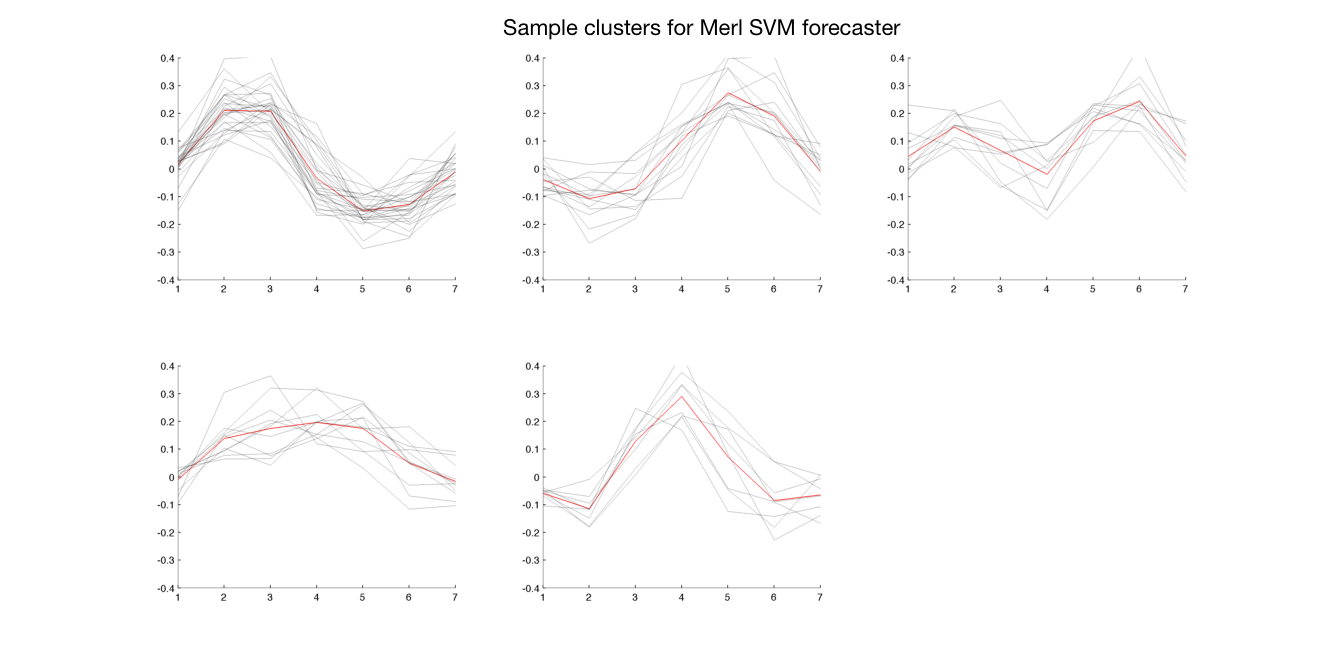
\includegraphics[width=1.00\textwidth]{merl_sample_clusters_svm.png}
	\end{center}
	\caption{Extracted residuals from the Merl dataset.  Data was taken from the top 10\% of the SVM forecaster's residuals.}
	\label{fig:merl_clusters}
\end{figure}

\begin{figure}
	\begin{center}
		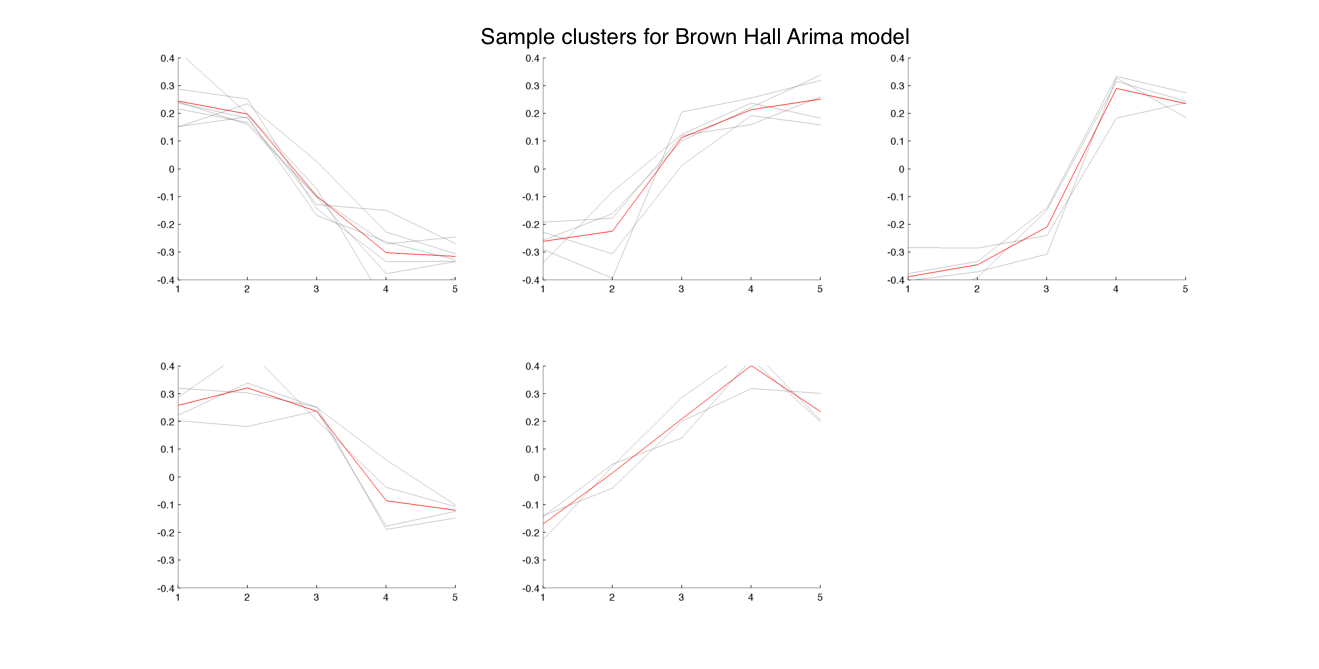
\includegraphics[width = 1.0\textwidth]{brown_sample_clusters_arima.png}
	\end{center}
	\caption{Extracted residuals from the Brown dataset.  Data was taken from the top 15\% of the Arima forecaster's residuals.}
	\label{fig:brown_clusters}
\end{figure}

\ref{fig:brown_clusters} is the set of clusters from the Brown dataset extracted from the Arima forecaster.  The clusters from the dataset were taken from the top 15\% of the Brown data residuals.  Notice how these clusters, unlike the clusters from \ref{fig:merl_clusters} do not begin nor end on zero.  This likely means that the true residuals are longer in length and those extracted.  However, our method of silhouette score maximization returned this set as the best.  Most likely this is due to non-consistent residual behavior if the extracted residual window is increased.
  
\begin{figure}
	\begin{center}
		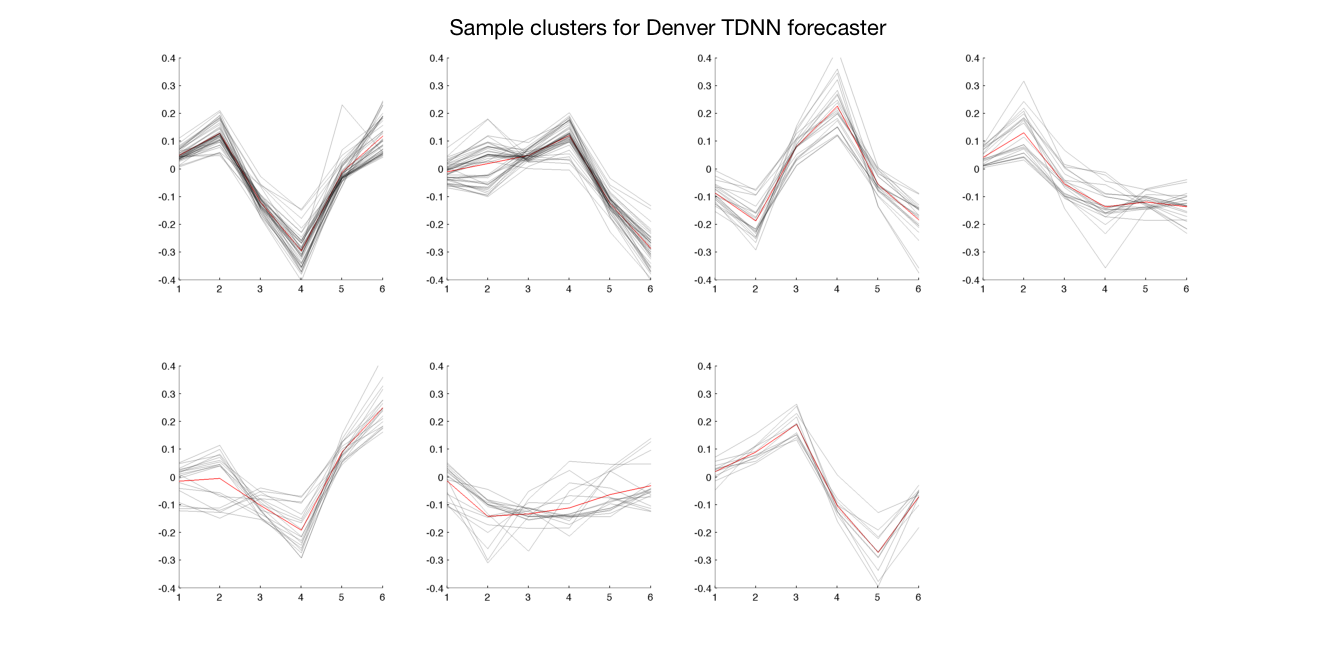
\includegraphics[width=1.0\textwidth]{denver_sample_clusters_tdnn.png}
	\end{center}
	\caption{Extracted residuals from the Denver dataset.  Data was taken from the top 10\% of the TDNN forecaster's residuals.}
	\label{fig:denver_clusters}
\end{figure}

\ref{fig:denver_clusters} displays the set of modeled clusters from the Denver dataset extracted from the TDNN forecaster.  These clusters were taken from the top 10\% of the forecaster's residuals.  Unlike in the extracted clusters of MERL and Brown, these clusters appear to have "sharp" transition.  This is likely due to the data being aggregated every 30 minutes instead of every 10 minutes like the other dataset.  Also, some of the clusters begin or end with a 0 residual, but others drift higher or lower.  Such a clustering is likely a scenario where modeling these clusters through a non-fixed technique may lead to better results.


\subsection{ABCF Derived}
\label{sec:abcf}
Here we present the math behind our Anomaly Bayesian combined forecasting algorithm.  Similar to the Bayesian combined forecaster introduced in Chapter 4, our ABCF algorithm is recursive and computationally efficient.  

We present the algorithm using two anomaly event models $a$ and $b$ with a background model $c$.  Extending the algorithm to work for any number of algorithms is apparent from this presentation.  For our work, the models $a$ and $b$ are modeled anomalies from our time series mixture of Gaussians, however this derivation allows the models to be any of a stochastic time series model such that it is possible to compute $p(x_{t} | a^{(i)}_{t})$.  Also, the model $c$ is assumed to be a background model which allows for the computation of $p(c_{t}|x_{t})$.  

Let $a_{t}^{(i)} = $ the event that model $b$ is active at time $t$ at index $i$ and $b_{t}^{(i)} = $ the event that model $b$ is active at time $t$ at index $i$.  At any time $t$ we have one of ${a^{(i)}_{t}}$, ${b^{(i)}_{t}}$ or $c$.  From this we know that 

\begin{equation}
\sum_{i}^{len(a)} p(a_{t}^{(i)}|x_{t}, \ldots, x_{1}) + \sum_{i}^{len(b)} p(b_{t}^{(i)}|x_{t}, \ldots, x_{1}) + p(c_{t}|x_{t}, \ldots, x_{1}).
\end{equation}

The goal of this forecaster is then to find each of $p(a_{t + 1}^{(i + 1)})$, $p(a_{t + 1}^{(i + 1)})$, and $p(c_{t + 1}).$  Given these model likelihoods, we can then produce a final forecast in a way similar to BCF in chapter 4.

We know from Bayes rule 

\begin {equation}
p(a_{t + 1}^{(i + 1)}|x_{t + 1}, \ldots, x_{1}) =
		\frac{p(x_{t + 1}|a^{(i + 1)}_{t + 1}, x_{t}, \ldots, x_{1}) p(a_{t + 1}^{(i + 1)}|x_{t}, \ldots, x_{1})}
	       {p(x_{t + 1})}
\end{equation}

Thus to find $p(a_{t + 1}^{(i + 1)}|x_{t + 1}, \ldots, x_{1})$ we need to compute:
\begin{itemize}
	\item $p(x_{t + 1}|a^{(i + 1)}_{t + 1}, x_{t}, \ldots, x_{1})$
	\item $p(a_{t + 1}^{(i + 1)}|x_{t}, \ldots, x_{1})$
	\item $p(x_{t + 1})$
\end{itemize} 

Computing $p(x_{t + 1})$ is straight forward from the law of total probability

\begin{equation}
	\begin{split}
		p(x_{t + 1}) = \sum_{i}^{len(a) - 1}p(x_{t + 1}|a_{t + 1}^{(i + 1)}, x_{t}, \ldots, x_{1})
						   p(a_{t + 1}^{(i + 1)}|x_{t}, \ldots, x_{1}) + \\
				      \sum_{i}^{len(b) - 1}p(x_{t + 1}|b_{t + 1}^{(i + 1)}, x_{t}, \ldots, x_{1}) 
						   p(b_{t + 1}^{(i + 1)}|x_{t}, \ldots, x_{1}) + \\
	        			      p(x_{t + 1}|c_{t + 1}, x_{t}, \ldots, x_{1})p(c_{t + 1}|x_{t}, \ldots, x_{1}).
	\end{split}
\end{equation}

The computation for $p(x_{t + 1}|a^{(i + 1)}_{t + 1}, x_{t}, \ldots, x_{1})$ is performed directly by computing the likelihood of a new data point $x_{t + 1}$ for model $a$ at offset $i + 1$.

Finally, the calculation of $p(a_{t + 1}^{(i + 1)}|x_{t}, \ldots, x_{1})$ is from an earlier forecast and is what gives our algorithm its recursive nature.  We pass the posterior of all values of $a_{t}$ to the priors of $a_{t + 1}.$  Thus $p(a_{t + 1}^{(i + 1)}|x_{t}, \ldots, x_{1})$ is simply a passed value from the last time step in our algorithm.  Specifically we define 

\begin{equation}
	p(a_{t + 1}^{(i + 1)} | x_{t}, \ldots, x_{1}) = 
		\begin{cases}
			p(a_{t}^{(i)}|x_{t}, \ldots, x_{1}) & : i < len(a) \\
			0 & : otherwise.
		\end{cases}
	%\right
\end{equation}

Thus in the present of an event we pass along the likelihood of that even to the next time step and recompute the posterior of that event.  The prior for the start of each event is a user tunable parameter.  

\begin{equation}
	\begin{split}
		p(a_{t + 1}^{(1)}|x_{t}, \ldots, x_{1}) = p(a_{t + 1}^{(1)}) = \theta_a \\
		p(b_{t + 1}^{(1)}|x_{t}, \ldots, x_{1}) = p(b_{t + 1}^{(1)}) = \theta_b
	\end{split}
\end{equation}


%%%%%%%%%%%%%%%%%%%%%%%%%%%%%%%%%%%%%%%%%%%%%%%%%
%Demonstration of ABCF
%%%%%%%%%%%%%%%%%%%%%%%%%%%%%%%%%%%%%%%%%%%%%%%%%

\begin{figure}[!t]
	\begin{center}
		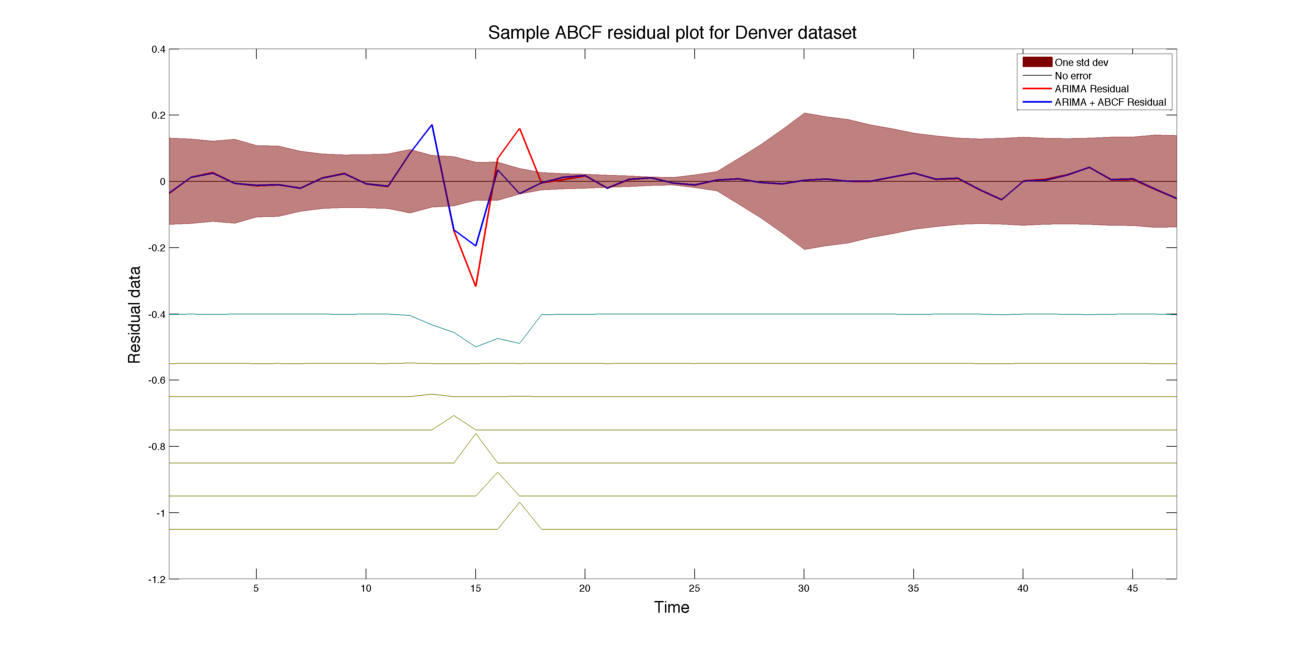
\includegraphics[width=1.0\textwidth]{sample_residual_plot_dataset_Denver.png}
	\end{center}
	\caption{Sample residual and the respective probabilities of each time step for the base forecaster and the a single activity model.}
	\label{fig:sample_abcf_residual}
\end{figure}

\subsection{Demonstration of ABCF}
\ref{fig:sample_abcf_residual} is a demonstration of ABCF.  This figure displays one sample time frame (in blue) from the Denver dataset along with the corresponding region for one standard deviation of noise from a best fit ARIMA forecaster with a horizon of two time steps.  The teal line below the graph is the likelihood of the background ARIMA model accurately representing the residual data from the set of clustered anomalies.  The remaining tan lines are the individual likelihoods of each time step of a given clustered anomaly \ref{fig:sample_cluster}  

The red line is the resulting ABCF forecast to the residual.  Ideally the residual should be completely zero, thus resulting in no forecasting error.  At approximately time 10, an anomalous event begins to occur.  The ABCF algorithm takes a few time steps to identify this anomaly and determine that the background ARIMA forecaster is no longer accurate.  We see this effect by noticing the teal line's reduction in likelihood from approximately time step 12 to time step 15.  During this time all other extracted clusters are attempting to fit the anomaly.

\begin{wrapfigure}{R}{0.3\textwidth}
\centering
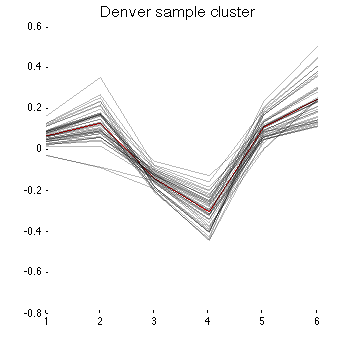
\includegraphics[width=0.25\textwidth]{denver_sample_cluster.png}
\caption{Extracted sample clustered anomaly.}
\label{fig:sample_cluster}
\end{wrapfigure}

The recursive nature of our likelihood time step propagation in the ABCF algorithm is apparent in the tan lines of this sample figure.  At time step 12, there is a slight perturbation in the top tan line.  This perturbation continues to rise both in value (indicating an increase in likelihood that this cluster is active) and time along the anomaly.  Finally at about time step 18, the model is finished.  At this point the likelihood of the background model begins to rise again and eventually the background model is once again the most prevalent model amongst all the extracted anomalies.

\ref{fig:sample_abcf_residual} displays a significant improvement in SQEONAN.  While the early stages of the anomaly show no improvement, the residual error during the middle of the anomaly is roughly halved and the residual error at the end of the anomaly is nearly zero.  \ref{fig:sample_abcf_denver} shows the final result of this forecast window.  This figure shows clearly how ABCF improves an ARIMA forecaster for this data segment during the later parts of an anomaly.

\begin{figure}[!h]
	\begin{center}
		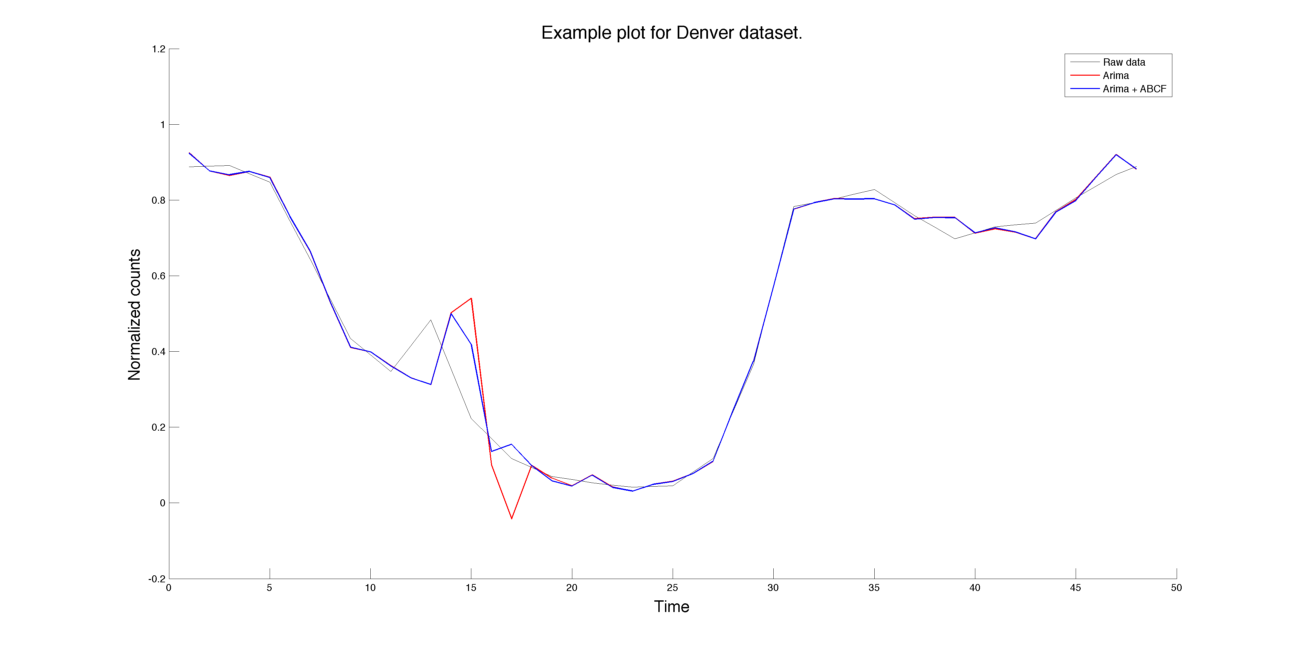
\includegraphics[width=1.0\textwidth]{sample_plot_Denver.png}
	\end{center}
	\caption{Two horizon time step results when applying ABCF to an ARIMA forecaster for a segment of the Denver dataset.}
	\label{fig:sample_abcf_denver}
\end{figure}


%%%%%%%%%%%%%%%%%%%%%%%%%%%%%%%%%%%%%%%%%%%%%%%%%
%Results of ABCF
%%%%%%%%%%%%%%%%%%%%%%%%%%%%%%%%%%%%%%%%%%%%%%%%%
\subsection{Results of ABCF}
Since the number of potential images to display about the improvements due to ABCF is quite large  we provide a few images here to demonstrate our results and put the remaining images in Appendix \ref{app:results} for the interested reader.

\bigskip
\noindent \textbf{Results per forecaster} 

%SQEONAN
\begin{figure}[!b]
	\begin{center}
		\subfigure[] {
			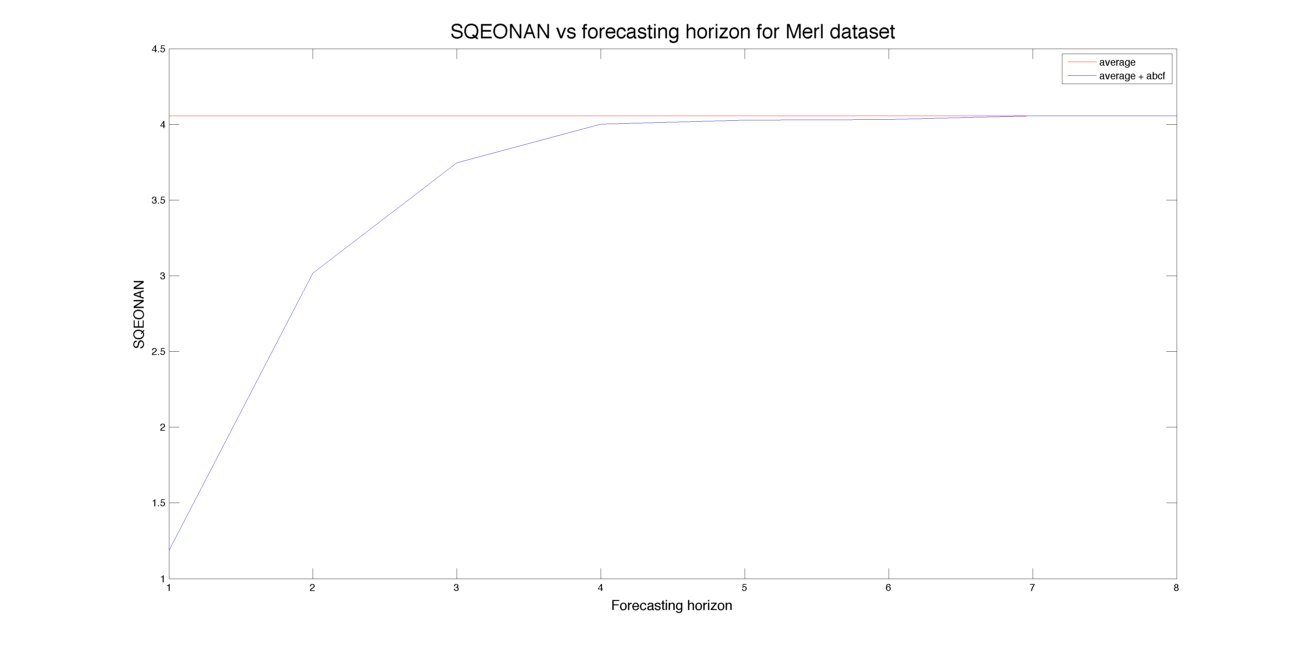
\includegraphics[width=0.49\textwidth]{sqe_merl_avg.png}
		}
		\subfigure[] {
			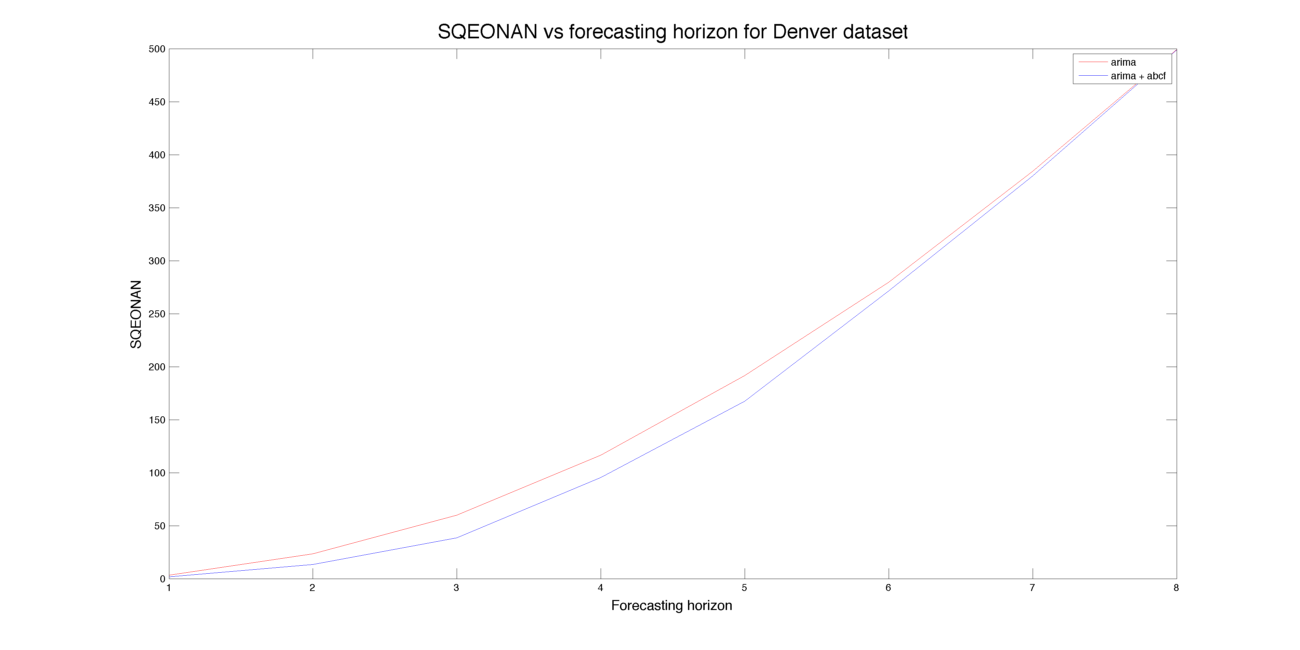
\includegraphics[width=0.49\textwidth]{sqe_denver_svm.png}
		} \\
		\subfigure[] {
			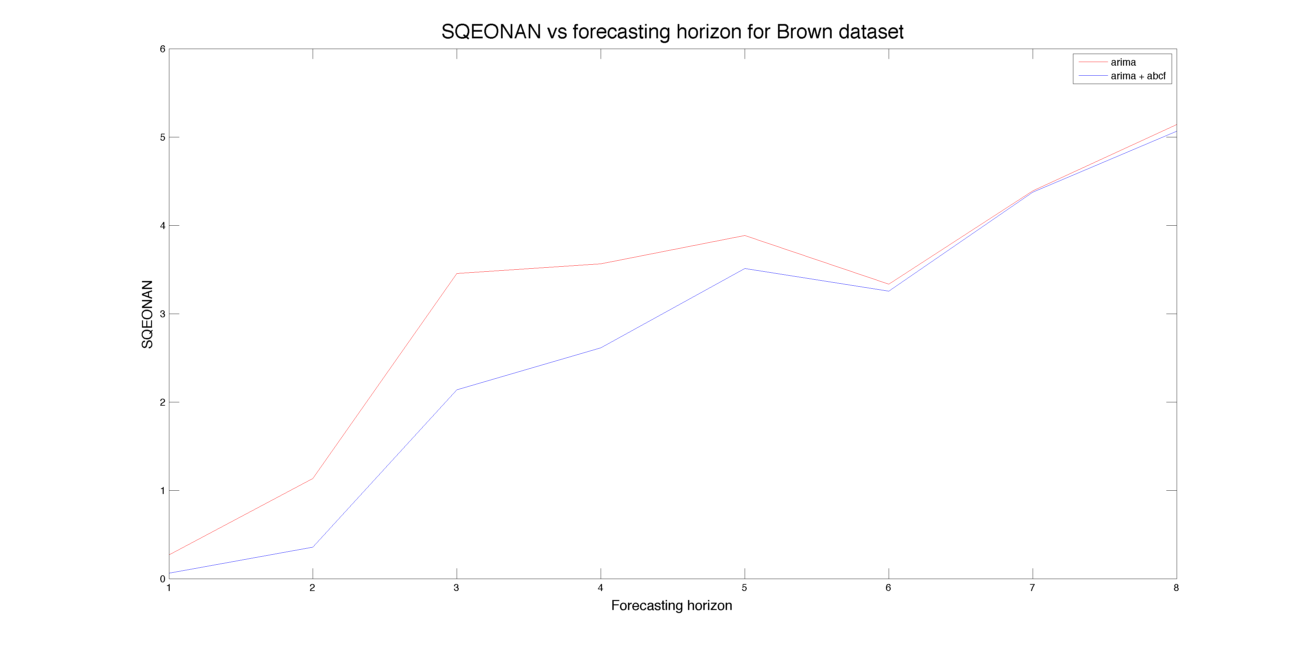
\includegraphics[width=0.49\textwidth]{sqe_brown_arima.png}
		}
		\subfigure[] {
			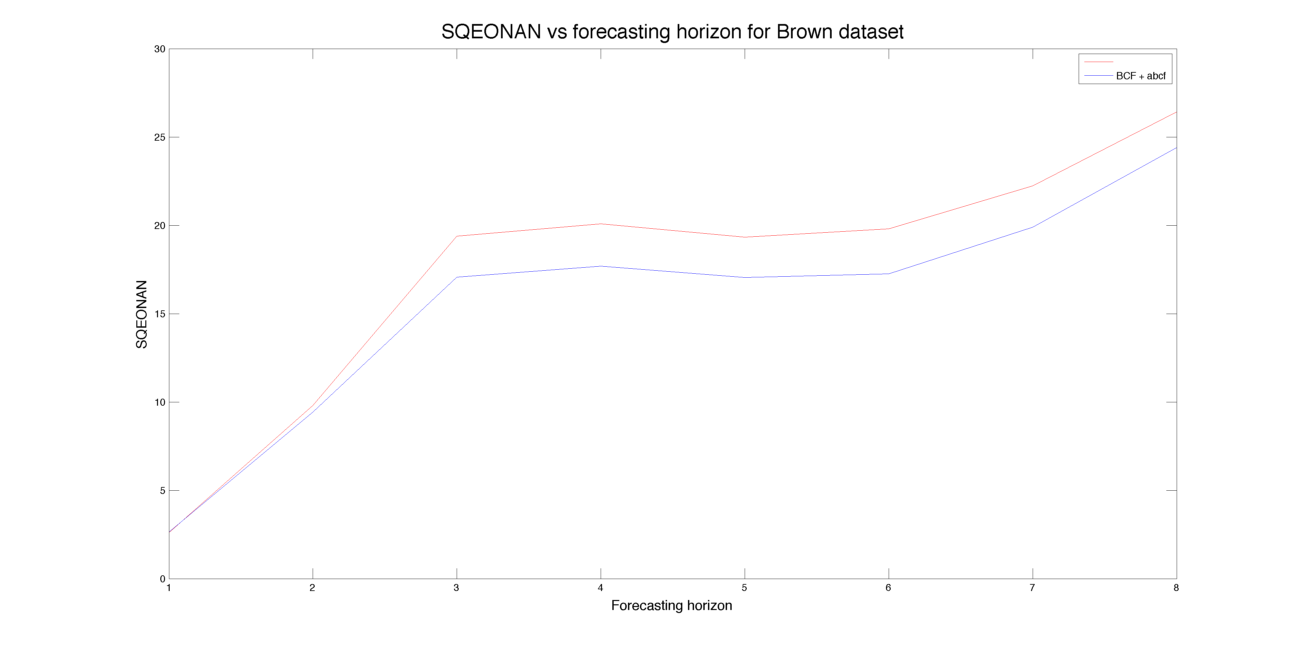
\includegraphics[width=0.49\textwidth]{sqe_brown_bcf.png}
		}
	\end{center}
	\caption{SQEONAN results of four sample forecasters with and without ABCF}
	\label{fig:sqe_results}
\end{figure}


%RMSE
\begin{figure}[!t]
	\begin{center}
		\subfigure[] {
			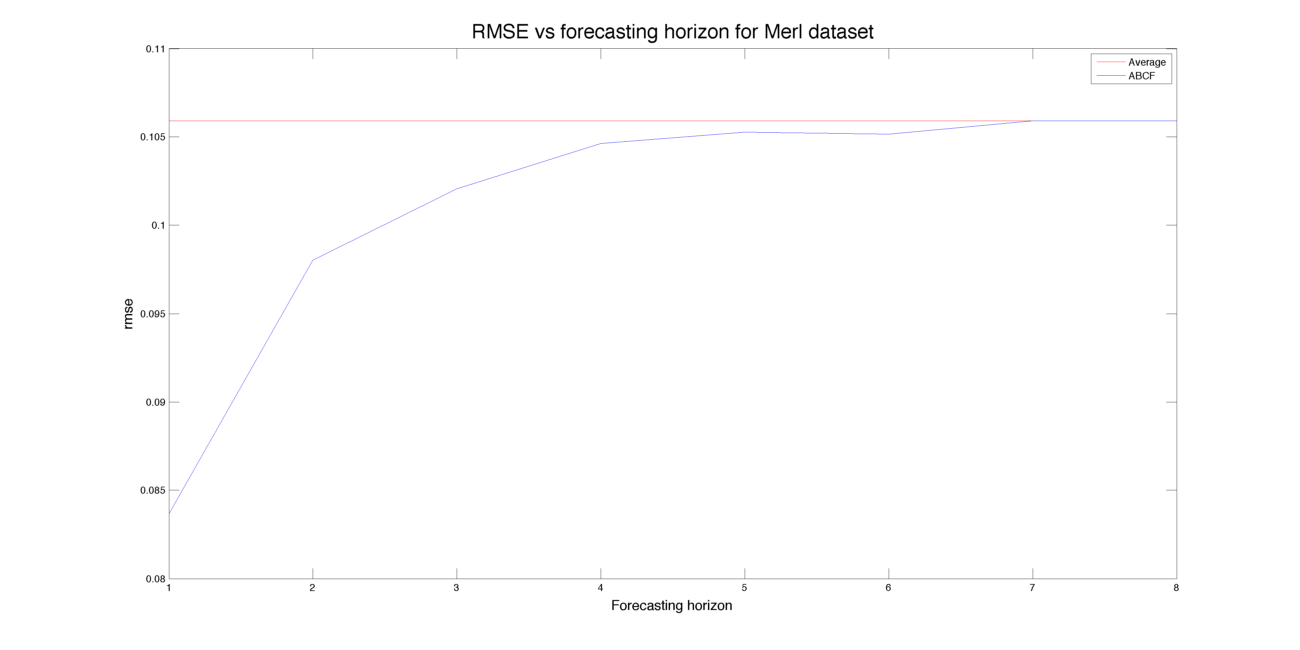
\includegraphics[width=0.49\textwidth]{rmse_merl_avg.png}
		}
		\subfigure[] {
			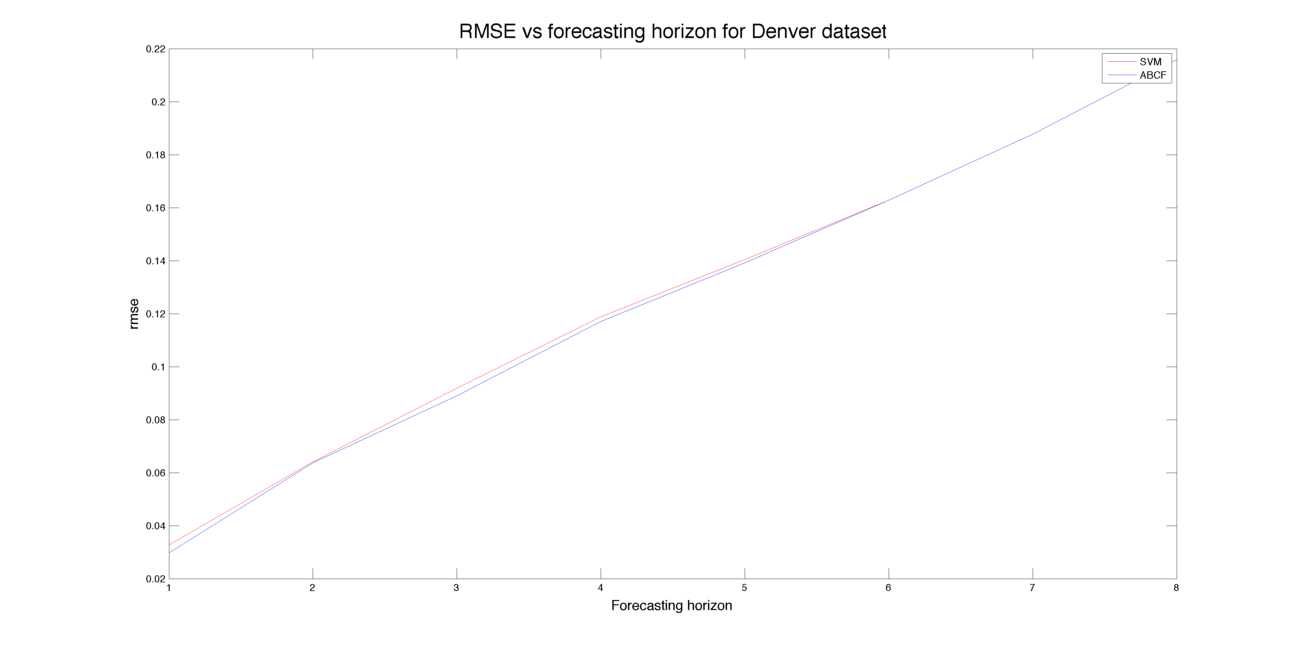
\includegraphics[width=0.49\textwidth]{rmse_denver_svm.png}
		} \\
		\subfigure[] {
			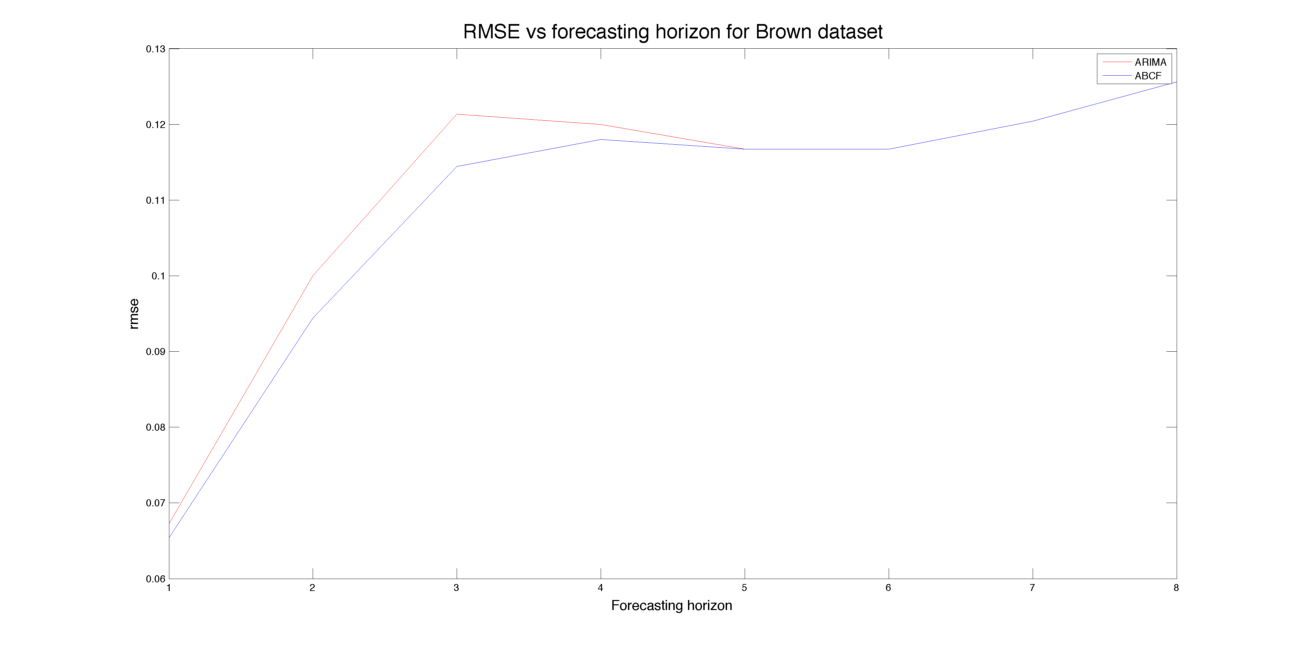
\includegraphics[width=0.49\textwidth]{rmse_brown_arima.png}
		}
		\subfigure[] {
			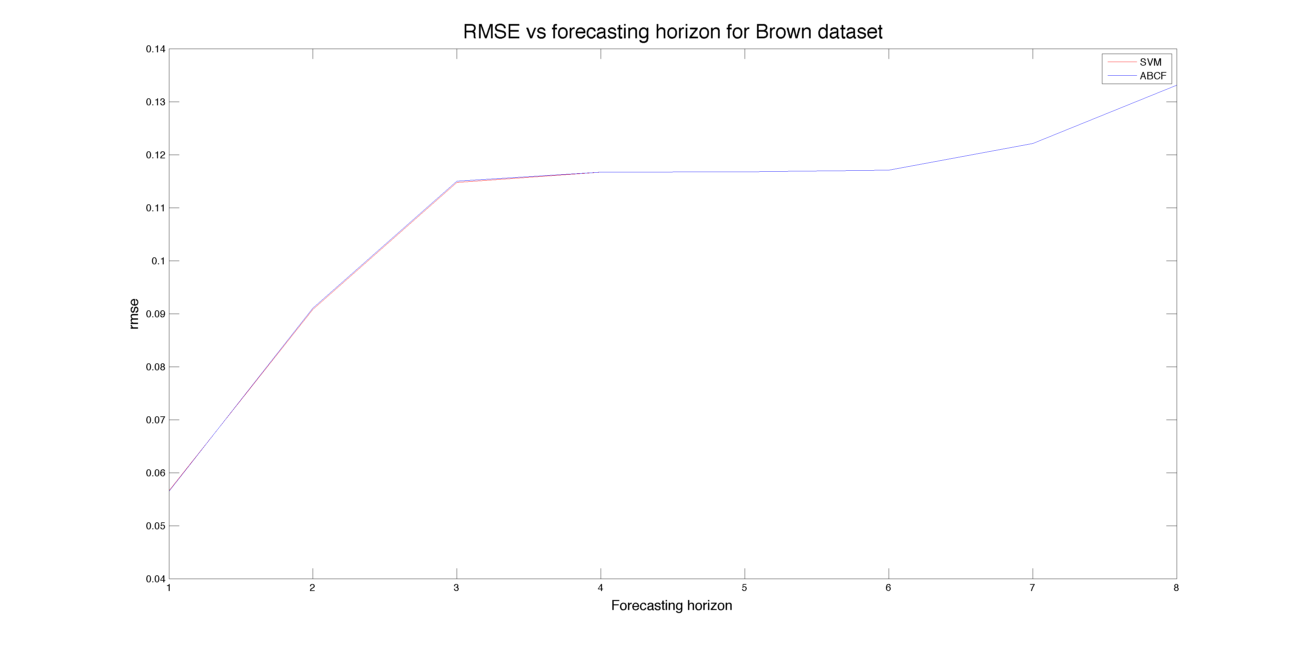
\includegraphics[width=0.49\textwidth]{rmse_brown_svm.png}
		}
	\end{center}
	\caption{RMSE results of four sample forecasters with and without ABCF}
	\label{fig:rmse_results}
\end{figure}

%MASE
\begin{figure}[!t]
	\begin{center}
		\subfigure[] {
			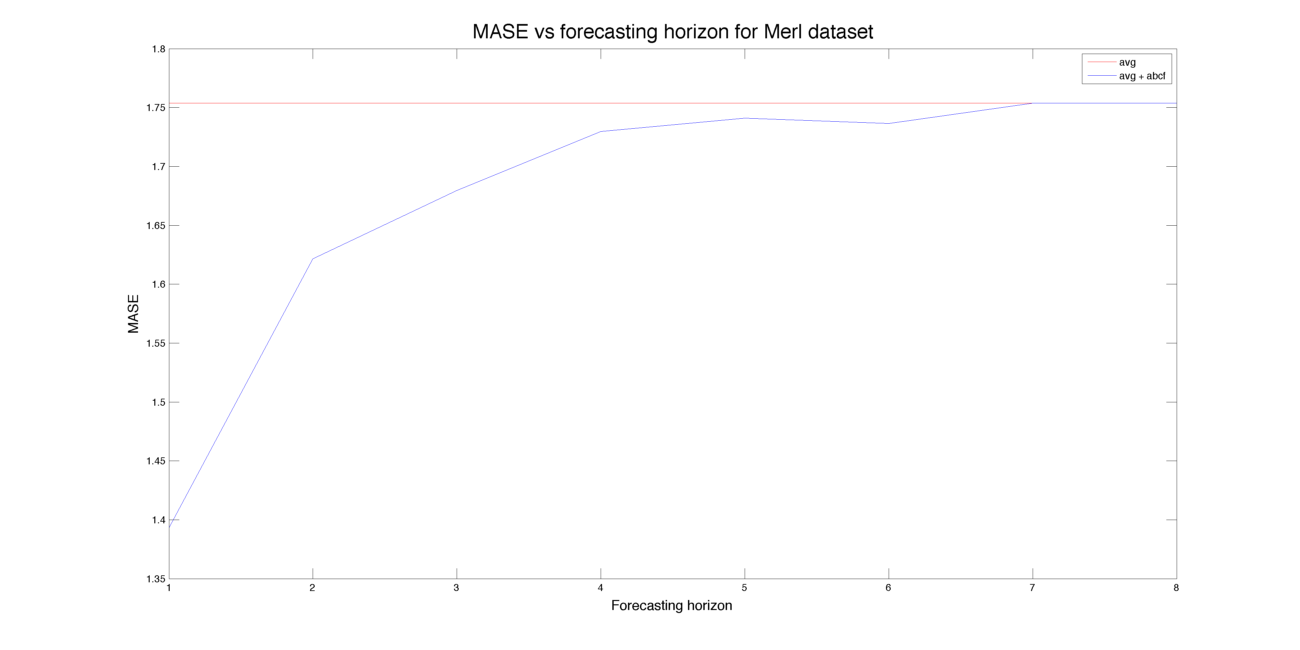
\includegraphics[width=0.49\textwidth]{mase_Merl_avg.png}
		}
		\subfigure[] {
			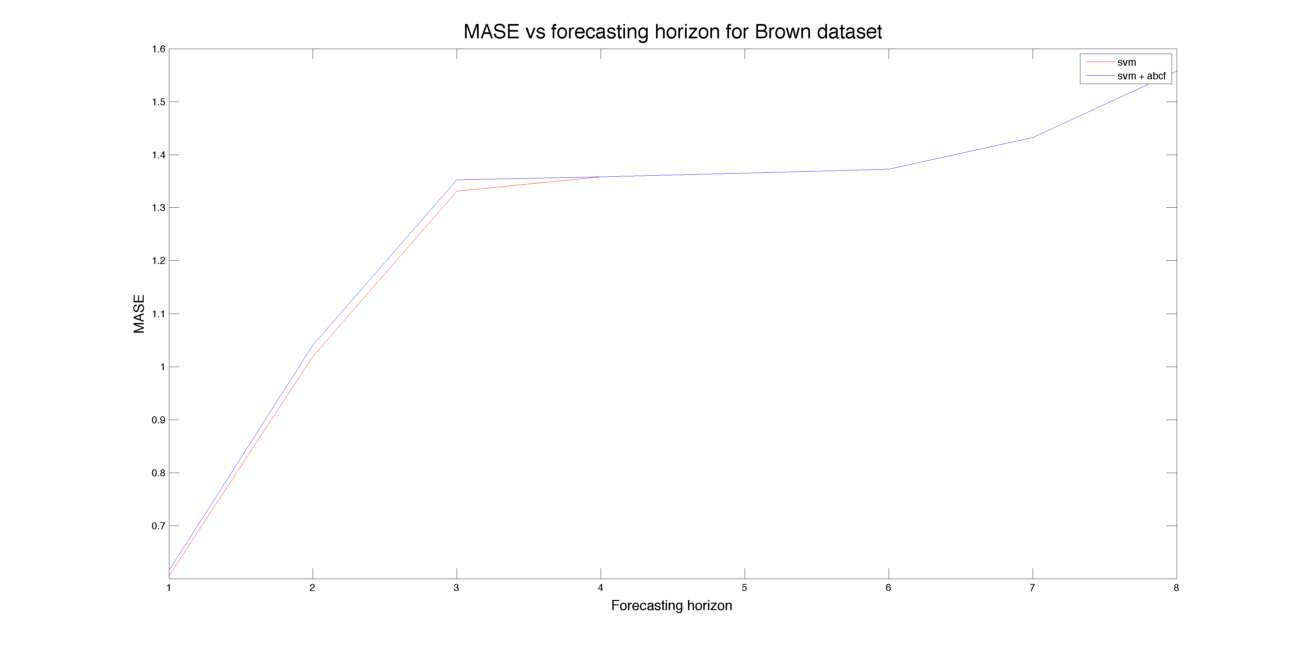
\includegraphics[width=0.49\textwidth]{mase_Brown_svm.png}
		} \\
		\subfigure[] {
			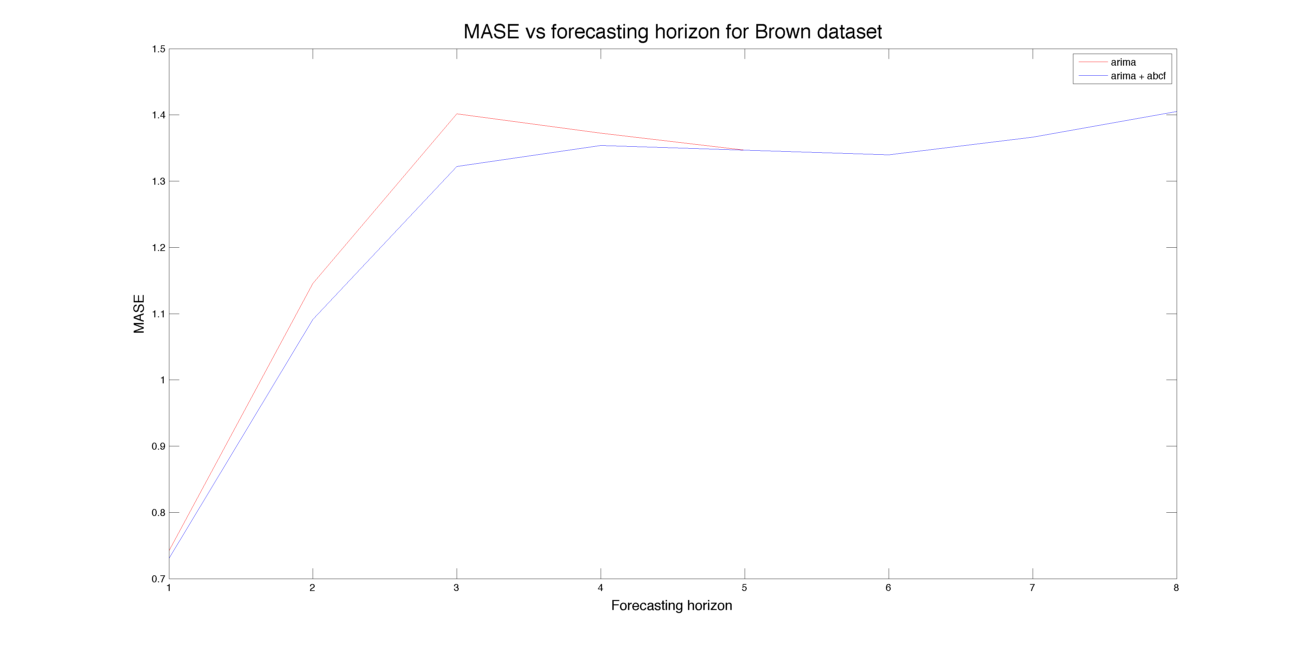
\includegraphics[width=0.49\textwidth]{mase_Brown_arima.png}
		}
		\subfigure[] {
			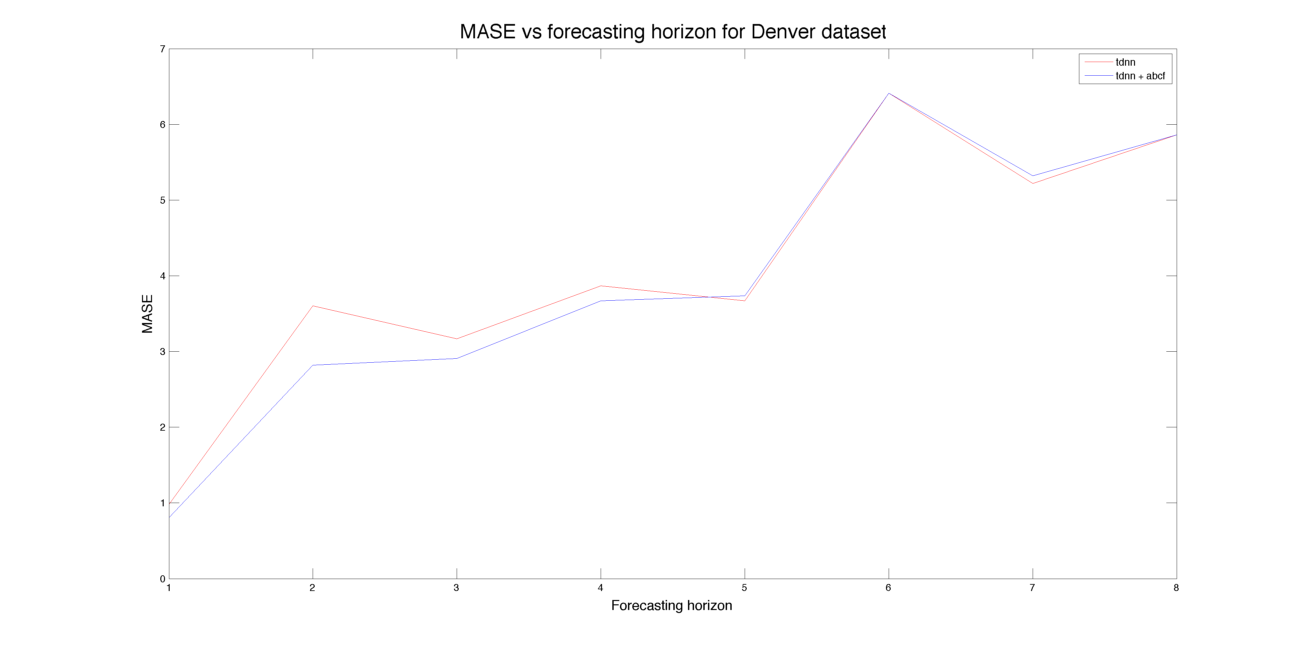
\includegraphics[width=0.49\textwidth]{mase_Denver_tdnn.png}
		}
	\end{center}
	\caption{MASE results of four sample forecasters with and without ABCF}
	\label{fig:mase_results}
\end{figure}

\ref{fig:sqe_results} demonstrate the improvements to the SQEONAN metric of applying our ABCF algorithm to each dataset for each activity model.  A set of sample RMSE and MASE results are given in \ref{fig:rmse_results} and \ref{fig:mase_results}.  In most of these figures, ABCF improves or is equal to the forecasting algorithm on its own for each forecasting horizon up to 15 time steps in the future.  Maximum total improvement is typically achieved between two and four time steps into the future.  Maximum percentage improvement is typically between one and two time steps into the future.

As ABCF is an ensemble forecaster, it can make no guarantees on its improvement.  \ref{fig:sqe_results}(d) and \ref{fig:mase_results}(d) demonstrate cases where ABCF performed worse than simply the base forecaster.  For forecasts one time step ahead on the Brown Hall dataset, the BCF forecaster out performed a hybrid BCF + ABCF forecast.  From our results, we found that such negative effects on forecasting performance were rare, occurring in only a few of our examples.

\ref{fig:rmse_results} and \ref{fig:mase_results} demonstrates the results of ABCF applied to the same some of the same datasets from \ref{fig:sqe_results}.  Notice that in most cases, there are significantly smaller improvements in both MASE and RMSE than that measured with SQEONAN.  This result is expected.  ABCF improves forecasting during the presence of anomalies.  Due to the nature of anomalies being sufficiently rare, ABCF may not improve overall forecasting accuracy by a large margin.  \ref{fig:rmse_results}(b) and (d) show almost no difference.  

\newpage



%%%%%%%%%%%%%%%%%%%%%%%%%%%%%%%%%%%%%%%%%%%%%%%%%
%Aggregated Results
%%%%%%%%%%%%%%%%%%%%%%%%%%%%%%%%%%%%%%%%%%%%%%%%%
\bigskip
\noindent \textbf{Aggregated Results} 

\begin{figure}[!b]
	\begin{center}
		\subfigure[] {
			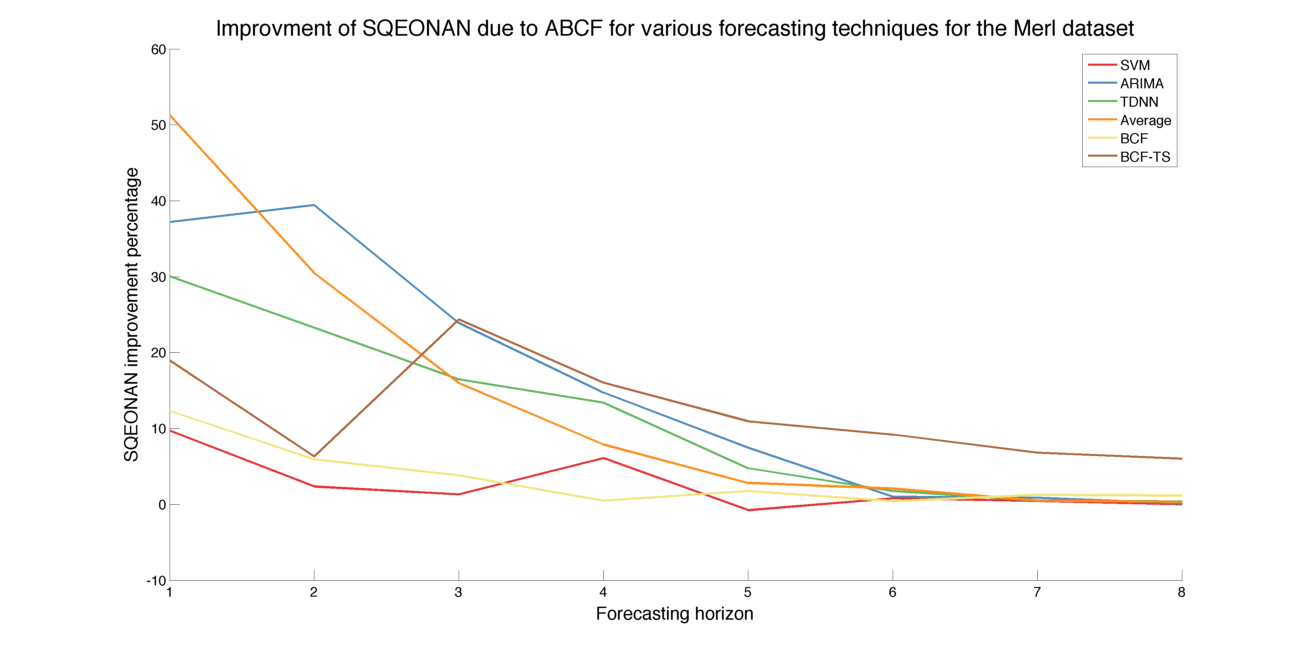
\includegraphics[width=0.49\textwidth]{sqeonan_improvement_for_each_forecaster_for_Merl.png}
		}
		\subfigure[] {
			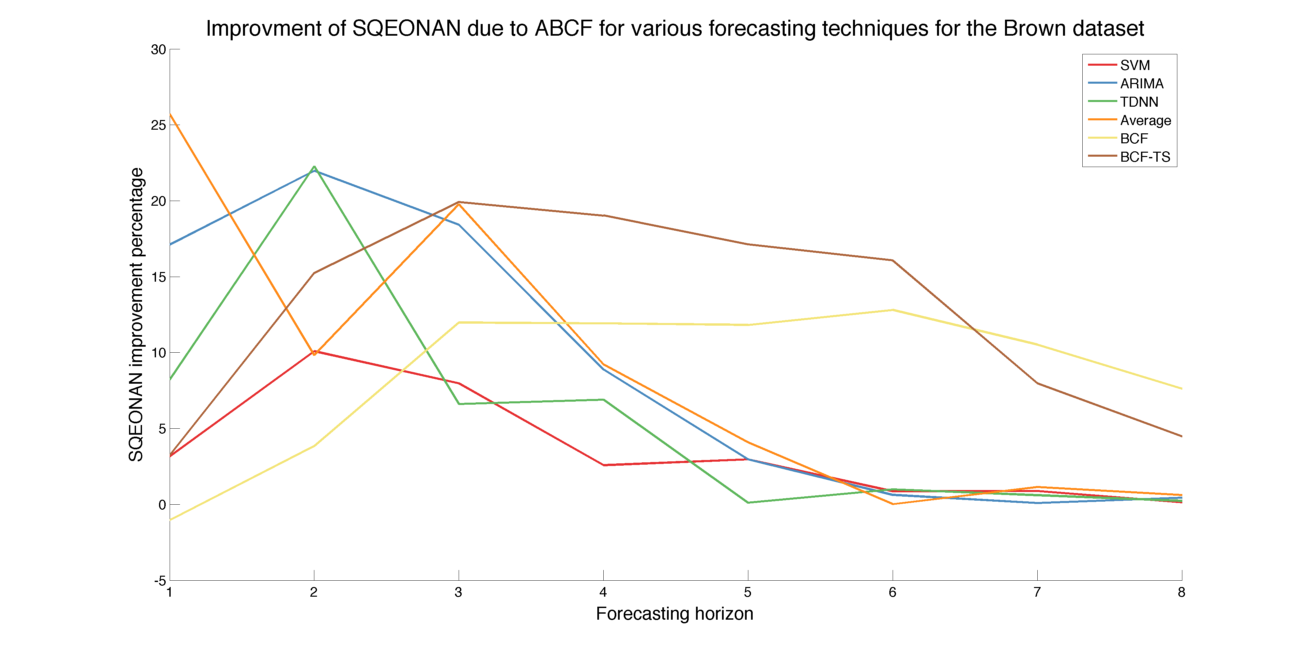
\includegraphics[width=0.49\textwidth]{sqeonan_improvement_for_each_forecaster_for_Brown.png}
		} \\
		\subfigure[] {
			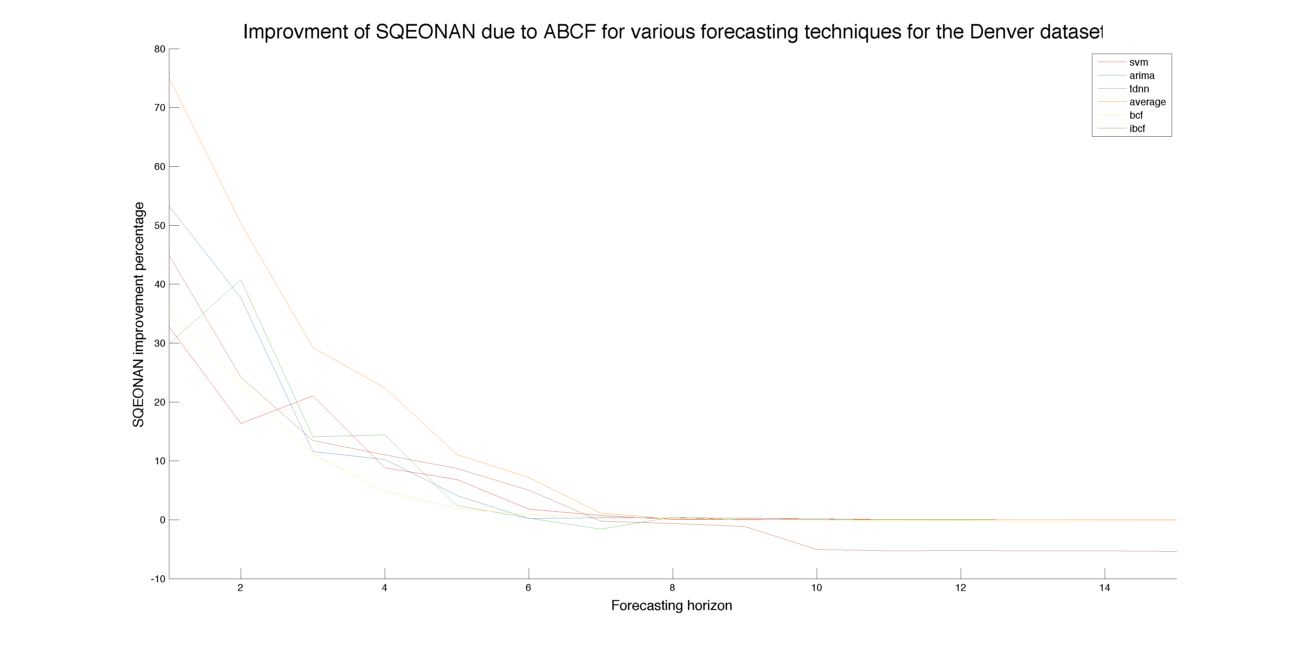
\includegraphics[width=0.49\textwidth]{sqeonan_improvement_for_each_forecaster_for_Denver.png}
		}
	\end{center}
	\caption{Percentage improvement to SQEONAN due to application of ABCF}
	\label{fig:sqe_improvement_dataset}
\end{figure}

\ref{fig:sqe_improvement_dataset} shows the percentage improvement using ABCF to supplement a given base forecaster.  The improvement due to ABCF varies greatly based on both forecaster and dataset.  As expected, ABCF improves a historic average forecaster by the largest margin.  The improvement is over 70\% on the Denver dataset and still over 25\% on the Brown hall set.

Both BCF and our IBCF algorithm introduced in the last chapter appear to have the smallest margin for improvement.  In the case of the Denver dataset, forecasts more than 10 time steps in the future are negatively affected by ABCF.  We believe the smaller improvement margins are due the properties of ensemble forecasters.  Such forecasters will change forecasting models based on the structure of the dataset at any given time.  These changes may not lead to clusters which are clean and thus as easily able to be modeled.  (TODO back this up with silhouette scores)

TODO include selected RMSE and MASE results

TODO include overall average improvement

TODO include results of sqeonan with ABCF improvements vs a few other forecasters


\begin{figure}
	\begin{center}
		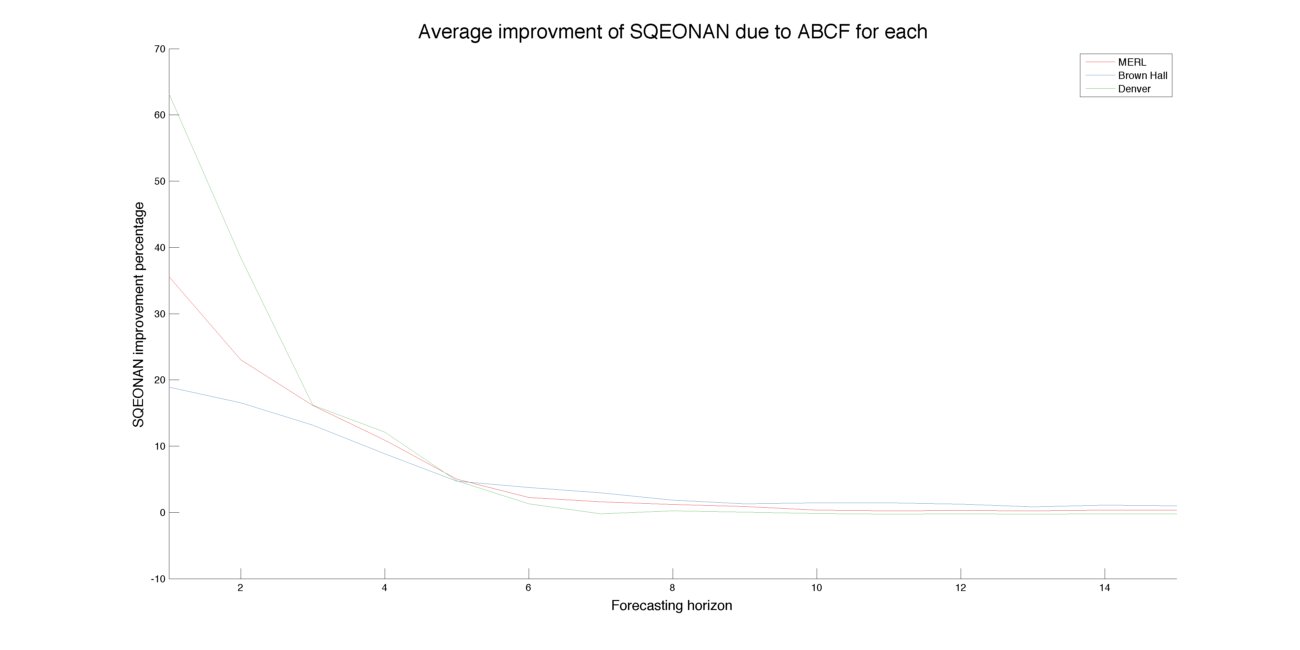
\includegraphics[width = 1.0\textwidth]{sqeonan_improvement_for_each_dataset.png}
	\end{center}
	\caption{Average percent improvement of applying ABCF to each forecaster to a given dataset.}
	\label{fig:sqeonan_improvement_all_dataset}
\end{figure}






%%%%%%%%%%%%%%%%%%%%%%%%%%%%%%%%%%%%%%%%%%%%%%%%%
%Future work
%%%%%%%%%%%%%%%%%%%%%%%%%%%%%%%%%%%%%%%%%%%%%%%%%
\subsection{Future unexplored work on ABCF}
While we are happy with the current status of the ABCF algorithm, we would recommend the following potential avenues for improvement.

\begin{enumerate}
	\item Explore different data extraction and clustering techniques.  More research into techniques which do not rely on fixed length extracted residual windows.  If a reliance on a sliding window extraction method is \texttt{•}o continue, then trimming or growing the sliding window based on the shape of any potential residual.  Another possibility would be to use a sparse dictionary encoding technique to determine the a best dictionary of anomalies for each residual time series.
	
	\item Acquire and test with other datasets.  The datasets presented here give a baseline to test from, but we realize that it does not represent all types of human traffic data.  We would like to test from a traffic dataset with shorter time scales (recall that the Denver dataset is every 30 minutes).  Also we would like to have other types of building data.  Do our approaches work with apartments or government buildings?  Rich building datasets would allow us to answer this question and may lead to improvements in our approach based on the results.
	
	\item Test with additional forecasters.  The four base forecasters we've selected represent a good base, but other forecasters, such as wavelet based or Markov based, may produce some unintuitive results.  We are especially interested in a forecaster or cluster which has a non-Gaussian noise distribution.  Our algorithm allows for any noise distribution, but all of our tests have only been with Gaussian noise.
\end{enumerate}

